\section{DESENHOS DE EXECUÇÃO (ENTREGA 4)}\label{sec:desenhos_execucao}

% Os desenhos são gerados por imagens/desenhos_execucao/gerar_desenhos.py. Para mudar uma cota, altere o script e rode de novo.

A partir desta entrega, a equipe passou a tratar o Tag\&Go como um produto a ser fabricado em série, e não mais como um protótipo. Os documentos das Seções~\ref{sec:desenhos_execucao} a~\ref{sec:controle_qualidade} supõem uma planta dimensionada para 20 mil dispositivos por mês, em dois turnos, volume compatível com a frota de uma grande rede (Seção~\ref{sec:escala_vertical}). A configuração é a revisada pelo DFMA na Entrega~3 (Tabela~\ref{tab:dfma_estrutura}), com as mudanças M1 a M8.

O projeto detalhado termina com os desenhos cotados e tolerados e com a configuração final refletida na estrutura do produto \cite{rozenfeld2006gestao}. Foram feitos sete desenhos, um para cada peça fabricada e um para o subconjunto do mecanismo, que somados ao desenho de conjunto da Entrega~3 cobrem todos os itens fabricados e montados (Tabela~\ref{tab:des_lista}).

\begin{table}[htbp]
    \centering
    \caption{Lista de desenhos da Entrega 4}
    \label{tab:des_lista}
    \footnotesize
    \renewcommand{\arraystretch}{1.3}
    \begin{tabularx}{\textwidth}{@{}
        >{\RaggedRight\arraybackslash}p{1.3cm}
        >{\RaggedRight\arraybackslash}p{1.5cm}
        >{\RaggedRight\arraybackslash}X
        >{\RaggedRight\arraybackslash}p{2.0cm}
        >{\centering\arraybackslash}p{1.1cm}
        >{\RaggedRight\arraybackslash}p{2.4cm}@{}}
        \toprule
        \textbf{Desenho} & \textbf{Código} & \textbf{Item} & \textbf{Tipo} & \textbf{Escala} & \textbf{Figura} \\
        \midrule
        DE-01 & TG-111 & Base da carcaça & Fabricado & 1:1 & Figura~\ref{fig:de01} \\
        DE-02 & TG-112 & Tampa & Fabricado & 1:1 & Figura~\ref{fig:de02} \\
        DE-03 & TG-113 & Suporte do mecanismo & Fabricado & 2:1 & Figura~\ref{fig:de03} \\
        DE-04 & TG-211 & Corpo da garra, com o pino e o revestimento & Fabricado & 1,5:1 & Figura~\ref{fig:de04} \\
        DE-05 & TG-312 & Braço dos ímãs & Fabricado & 4:1 & Figura~\ref{fig:de05} \\
        DE-06 & TG-412 & Guia de luz e subconjunto da tampa & Fabricado e montado & 5:1 & Figura~\ref{fig:de06} \\
        DE-07 & SC-01 & Subconjunto do mecanismo & Montado & 2:1 & Figura~\ref{fig:de07} \\
        -- & TG-000 & Conjunto geral & Montado & -- & Figura~\ref{fig:dfma_conjunto} \\
        \bottomrule
    \end{tabularx}
    \source{Elaborado pelos autores (2026).}
\end{table}

As cotas partem das superfícies que posicionam cada peça no conjunto. No suporte, por exemplo, a referência A é o plano dos pés, e todas as alturas do mecanismo foram cotadas a partir dele. As cotas das quais depende a liberação da peça receberam a marca CC (característica crítica) e voltam no plano de controle da Seção~\ref{sec:controle_qualidade}. O que não tem tolerância indicada segue a norma do processo: ISO 20457 nas peças injetadas \cite{iso20457}, ISO 8062-3 na garra fundida \cite{iso8062} e ISO 2768 no braço usinado \cite{iso2768}, com os símbolos geométricos da ISO 1101 \cite{iso1101}.

\subsection{Cadeia de tolerâncias da folga do ímã}
\label{subsec:des_cadeia}

A cota que mais pesou nos desenhos não pertence a nenhuma peça. É a folga de 0,20~mm entre o ímã e a prateleira do suporte, na posição de soltar, que resulta de uma cota do suporte e de duas definidas na montagem. A equipe calculou a variação pelo pior caso e pela soma estatística, os dois métodos de análise de tolerâncias citados por \citeonline{rozenfeld2006gestao} (Tabela~\ref{tab:des_cadeia}).

\begin{table}[htbp]
    \centering
    \caption{Cadeia de tolerâncias da folga entre o ímã e a prateleira}
    \label{tab:des_cadeia}
    \footnotesize
    \renewcommand{\arraystretch}{1.3}
    \begin{tabularx}{\textwidth}{@{}
        >{\RaggedRight\arraybackslash}X
        >{\centering\arraybackslash}p{2.2cm}
        >{\centering\arraybackslash}p{2.0cm}
        >{\RaggedRight\arraybackslash}p{4.6cm}@{}}
        \toprule
        \textbf{Cota} & \textbf{Nominal (mm)} & \textbf{Tolerância (mm)} & \textbf{Onde é garantida} \\
        \midrule
        Face inferior da prateleira ao plano dos pés & 14,50 & $\pm$0,05 & Molde do suporte (DE-03) \\
        Face superior do braço ao plano dos pés & 2,50 & $\pm$0,03 & Batente da prensa, no Posto~1 (DE-07) \\
        Face polar do ímã à face superior do braço & 11,80 & $\pm$0,03 & Gabarito de colagem FD-01, no Posto~0 \\
        \midrule
        \textbf{Folga, pelo pior caso} & \textbf{0,20} & \textbf{$\pm$0,11} & 14,50 $-$ 2,50 $-$ 11,80 \\
        \textbf{Folga, pela soma estatística} & \textbf{0,20} & \textbf{$\pm$0,07} & Raiz da soma dos quadrados \\
        \bottomrule
    \end{tabularx}
    \source{Elaborado pelos autores (2026).}
\end{table}

Com 20 mil subconjuntos por mês, a soma estatística descreve melhor o lote do que o pior caso, e por isso o desenho DE-07 fixou a folga em 0,20~$\pm$0,10~mm. O pequeno excesso do pior caso fica coberto pelo teste funcional, que confere a folga em todas as unidades. A cadeia também explica a decisão de tirar a altura do ímã da peça e passá-la ao gabarito: se ela dependesse da altura do ímã comprado e da profundidade do alojamento, a variação somaria mais duas parcelas, e nenhuma delas poderia ser corrigida na montagem.

\subsection{Desenhos}
\label{subsec:des_folhas}

As Figuras~\ref{fig:de01} a~\ref{fig:de07} trazem as folhas, em A4. Três decisões tomadas no detalhamento aparecem nelas. No suporte, o ponto de injeção foi levado para a borda da prateleira e as marcas de extração foram proibidas nela, porque a planicidade é a característica mais difícil de obter no poliacetal. Na garra fundida, a anodização prevista no conceitual foi trocada por vibroacabamento e conversão química, já que o banho ataca o pino de aço embutido e as ligas com muito silício anodizam mal. Na tampa, o furo do pino foi cotado a partir das mesmas bordas que a posicionam na base, e a cota de 30,00~mm até o eixo dos mancais repete a da garra (DE-04), de modo que as duas peças fecham a mesma cadeia.

\begin{landscape}
\begin{figure}[p]
    \centering
    \caption{Desenho de execução DE-01: base da carcaça (TG-111)}
    \label{fig:de01}
    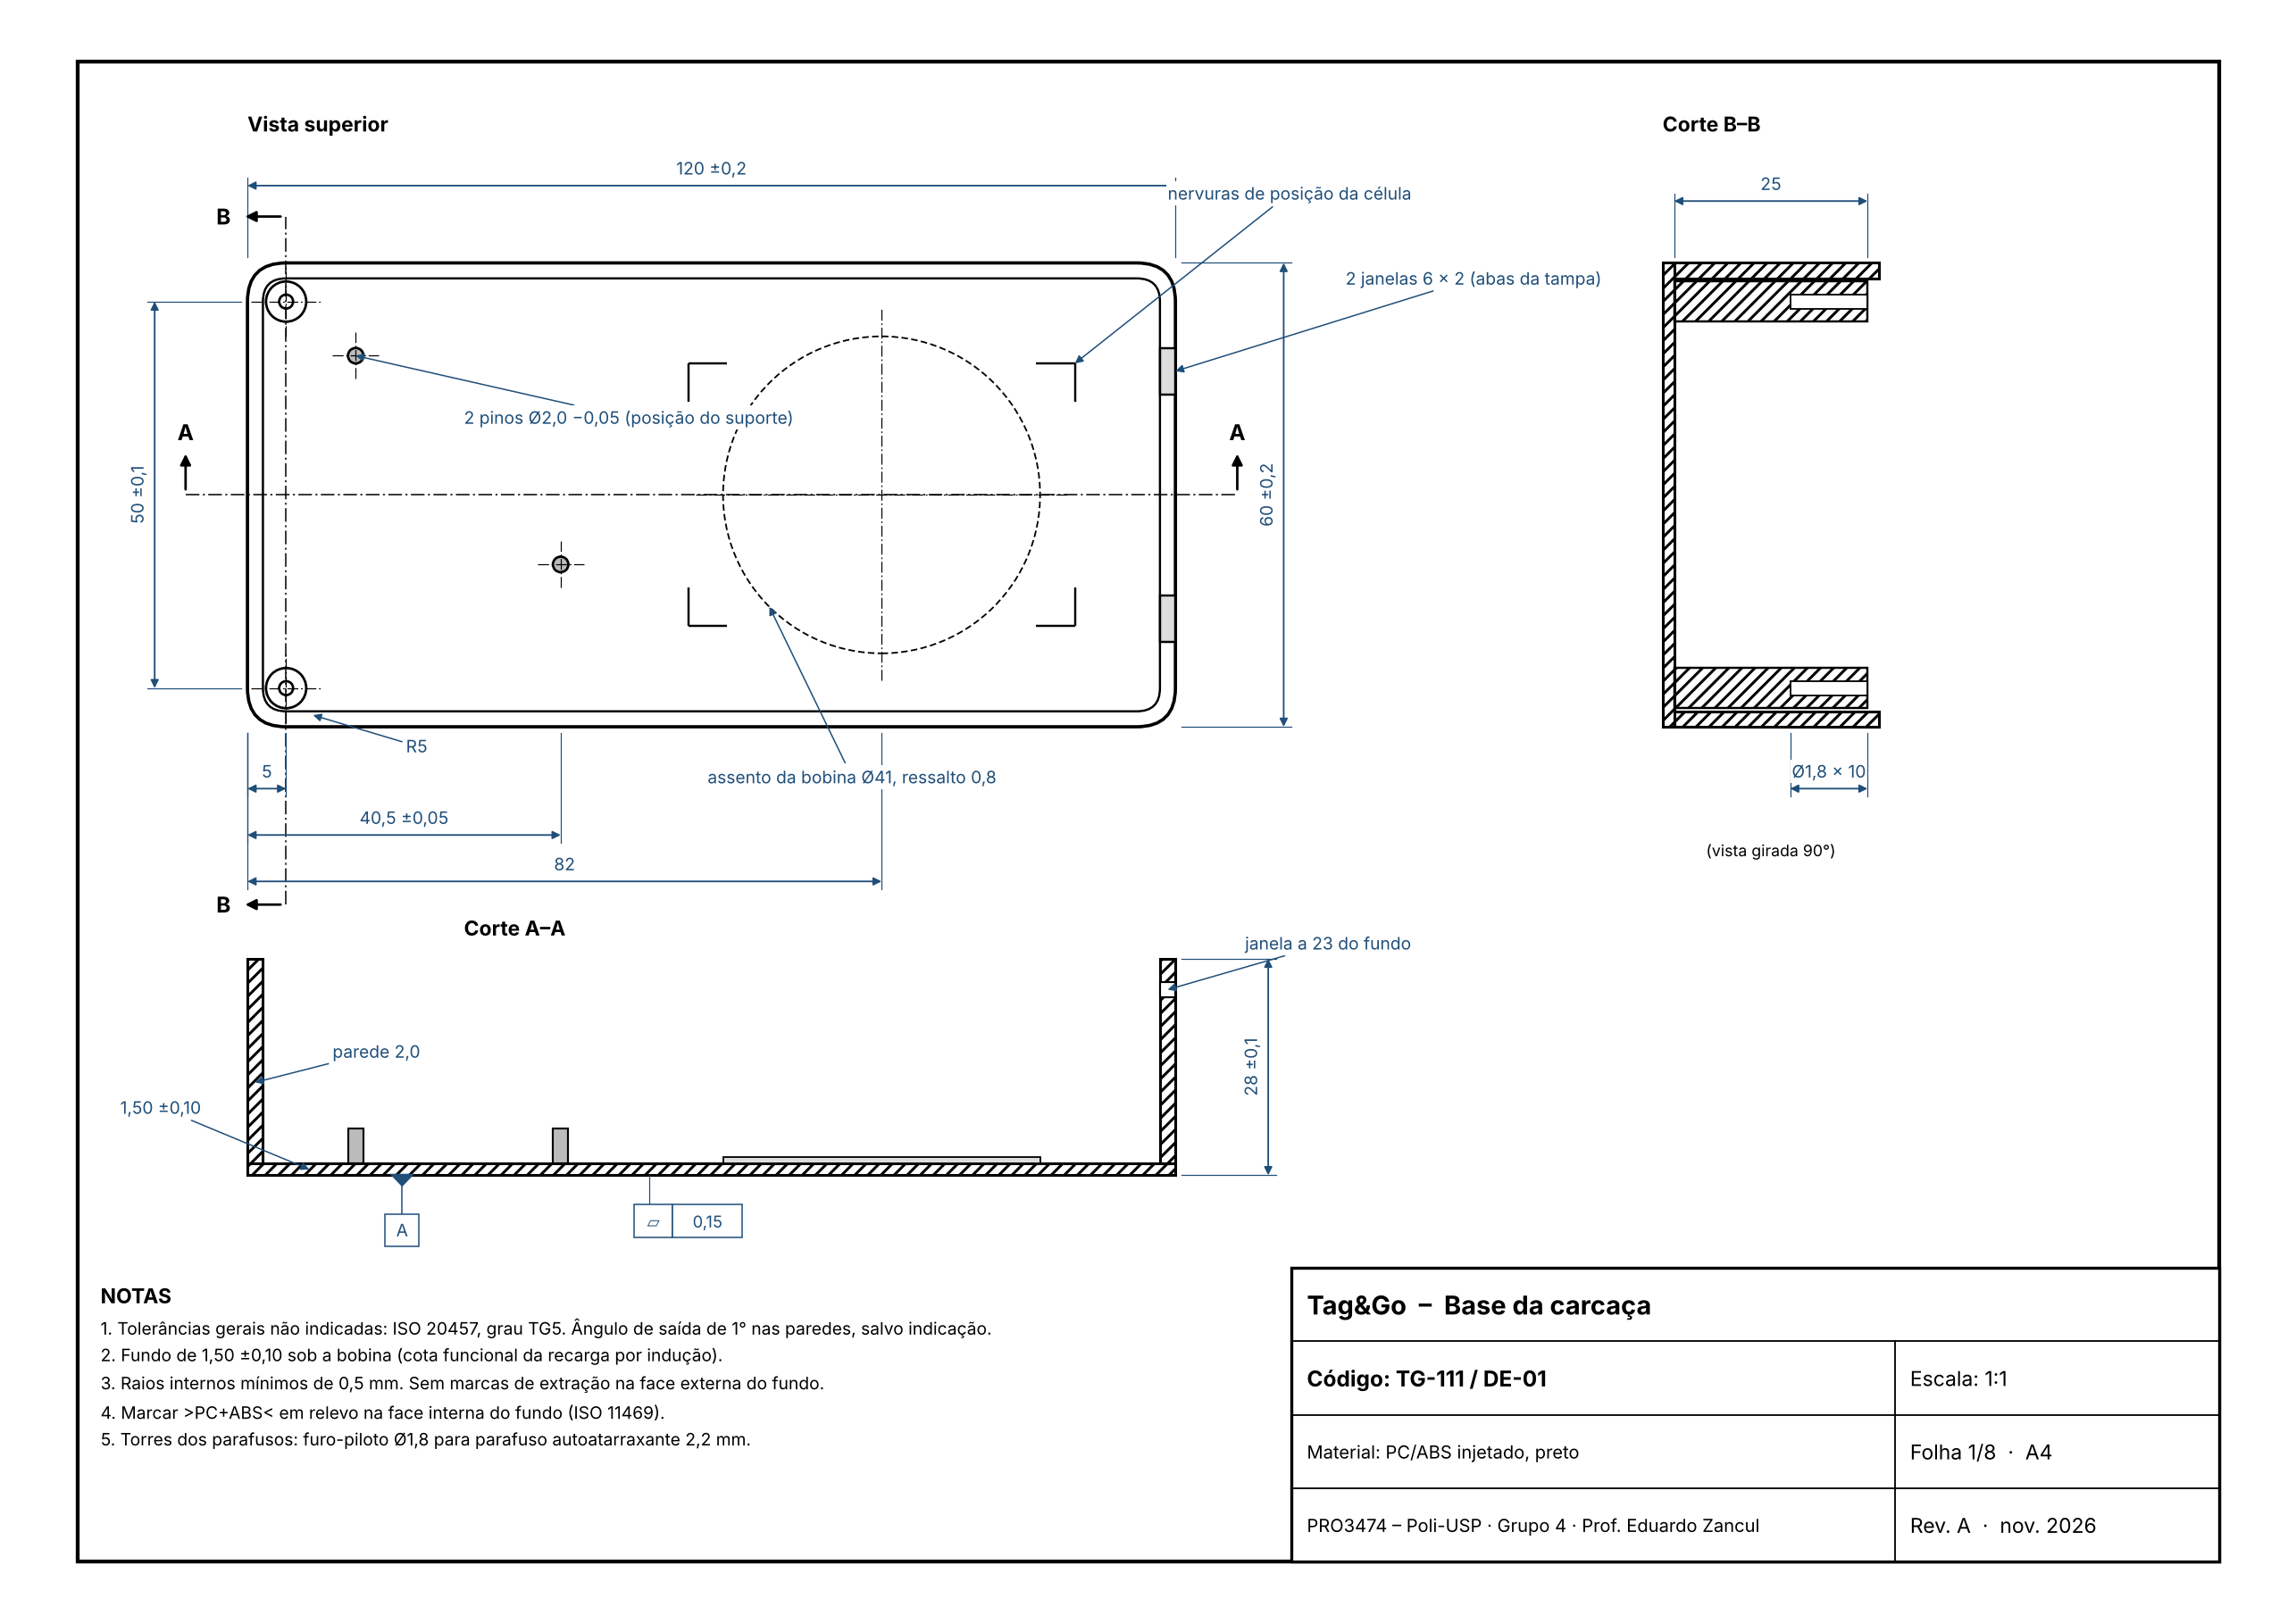
\includegraphics[height=0.86\textheight]{imagens/desenhos_execucao/de01_base.png}
    \source{Elaborado pelos autores (2026). Desenho gerado com apoio de ferramenta de IA.}
\end{figure}
\begin{figure}[p]
    \centering
    \caption{Desenho de execução DE-02: tampa (TG-112)}
    \label{fig:de02}
    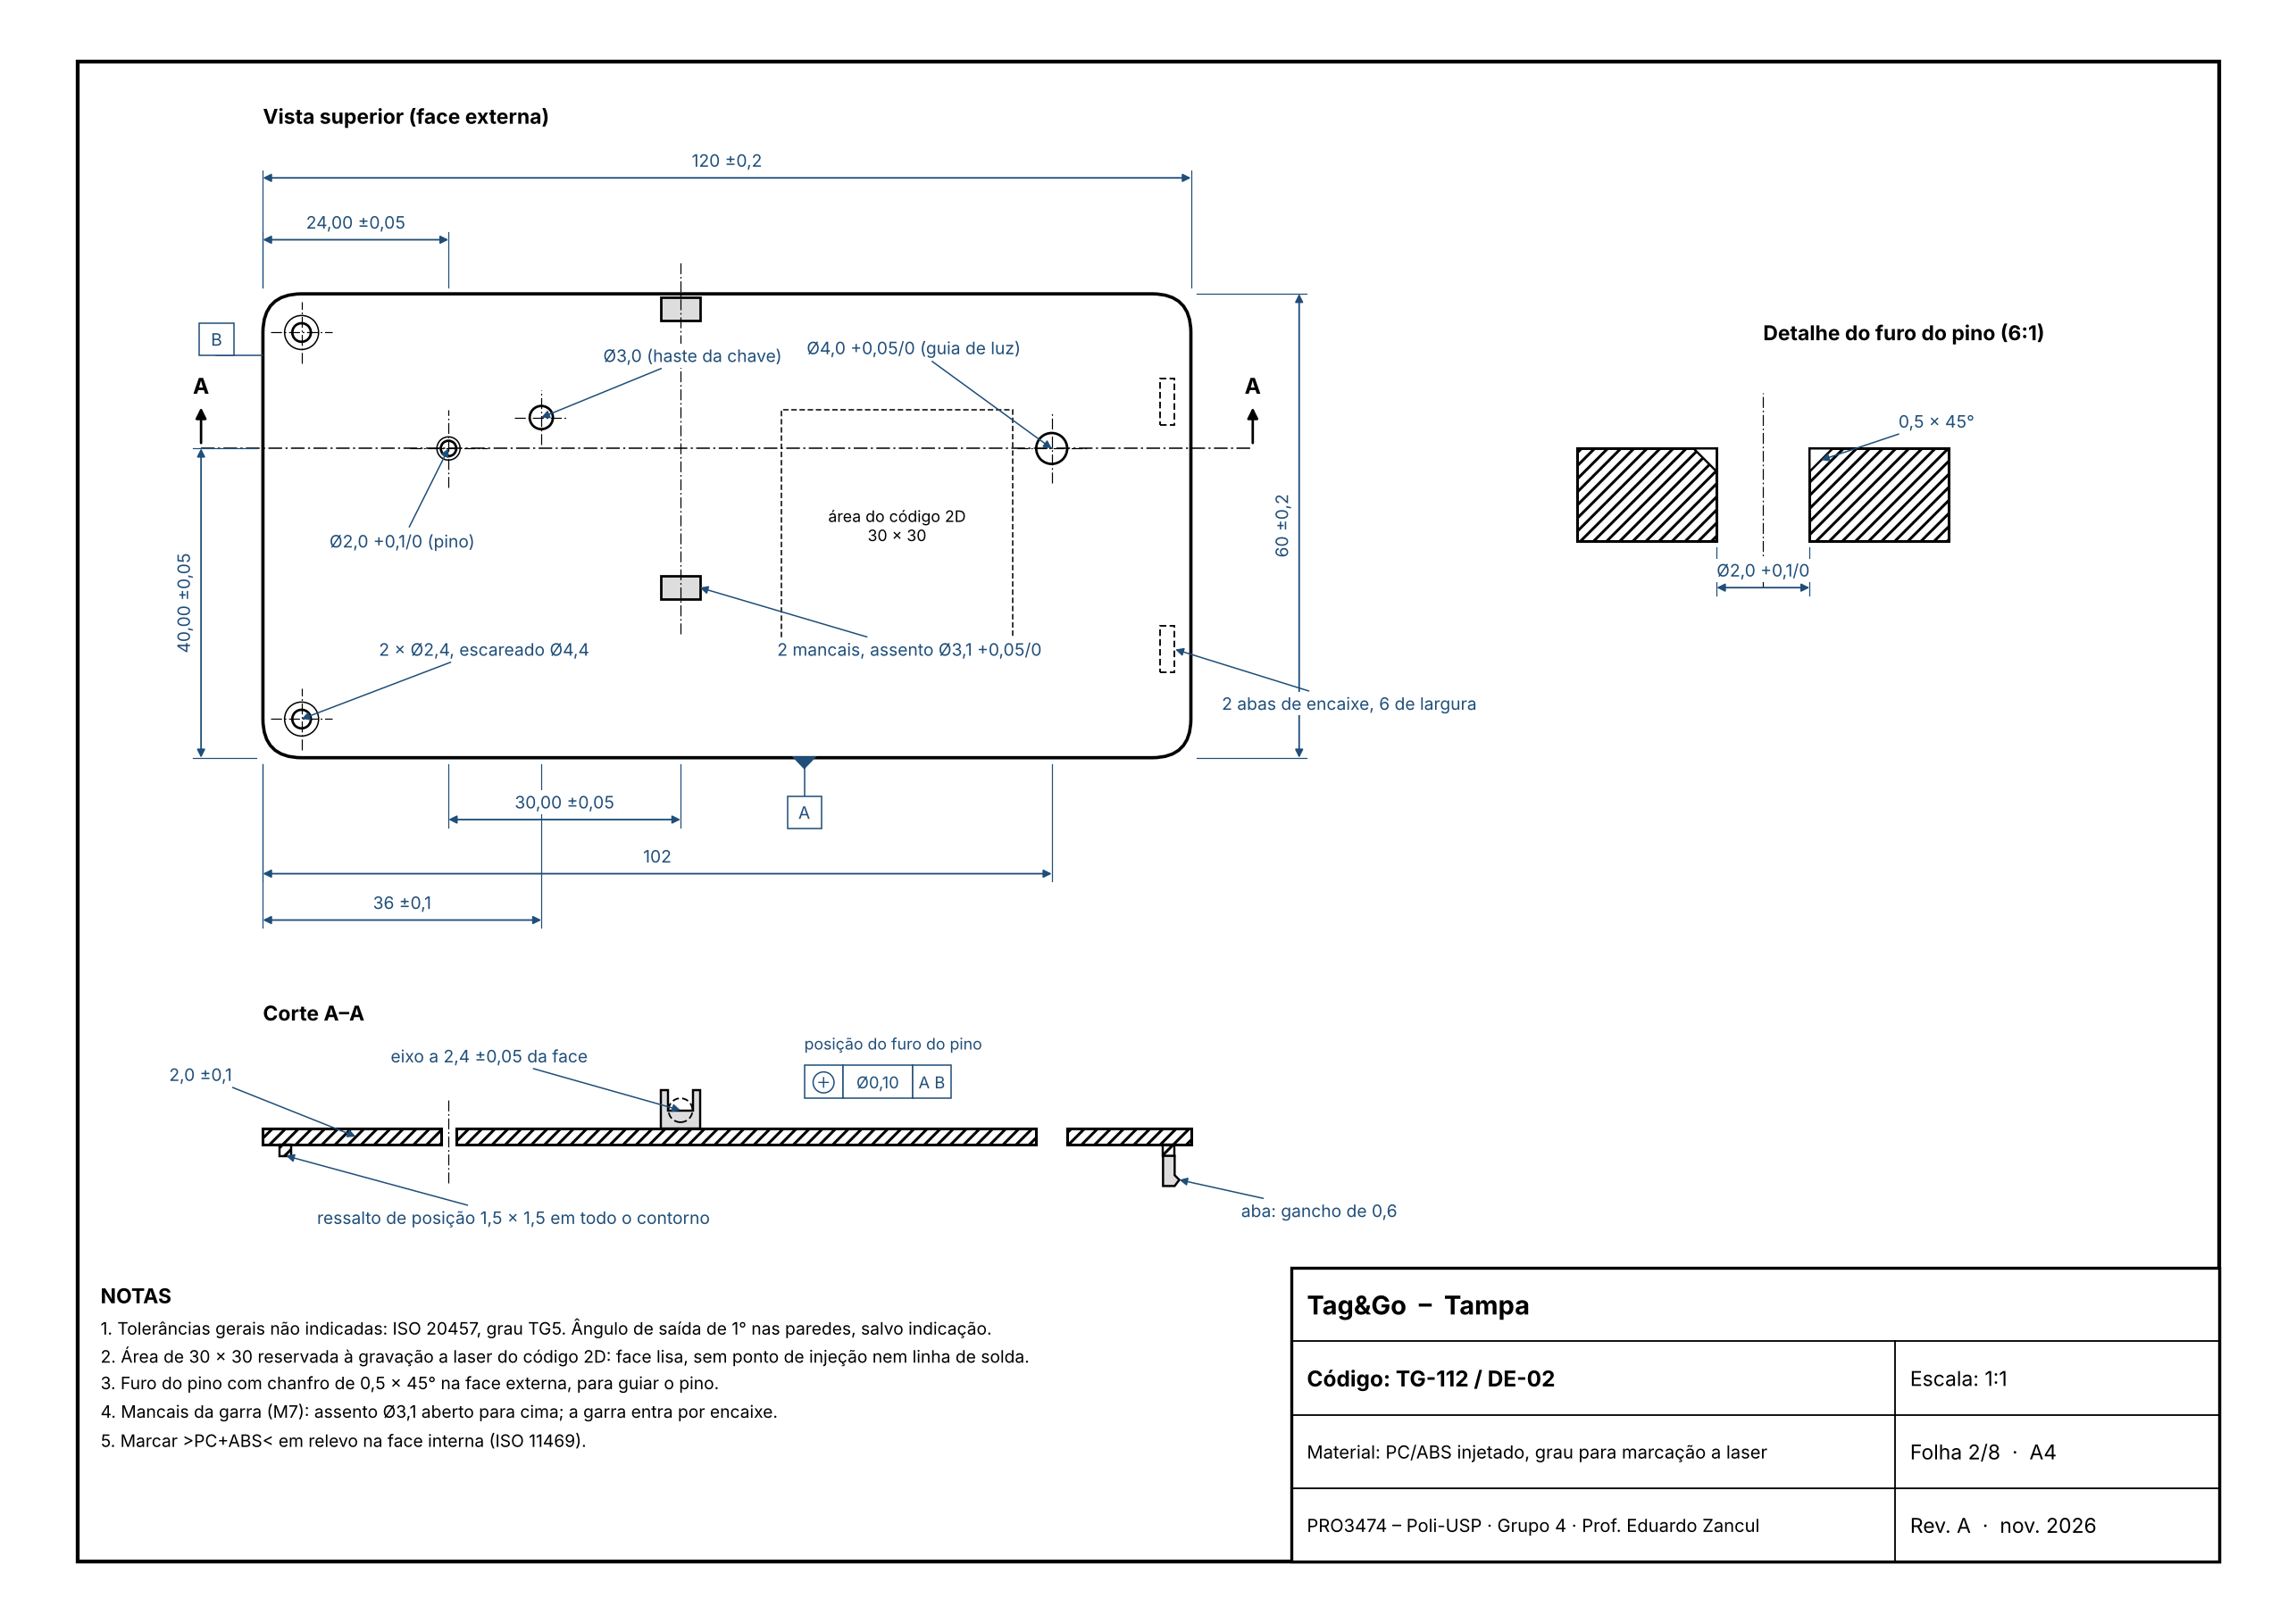
\includegraphics[height=0.86\textheight]{imagens/desenhos_execucao/de02_tampa.png}
    \source{Elaborado pelos autores (2026). Desenho gerado com apoio de ferramenta de IA.}
\end{figure}
\begin{figure}[p]
    \centering
    \caption{Desenho de execução DE-03: suporte do mecanismo (TG-113)}
    \label{fig:de03}
    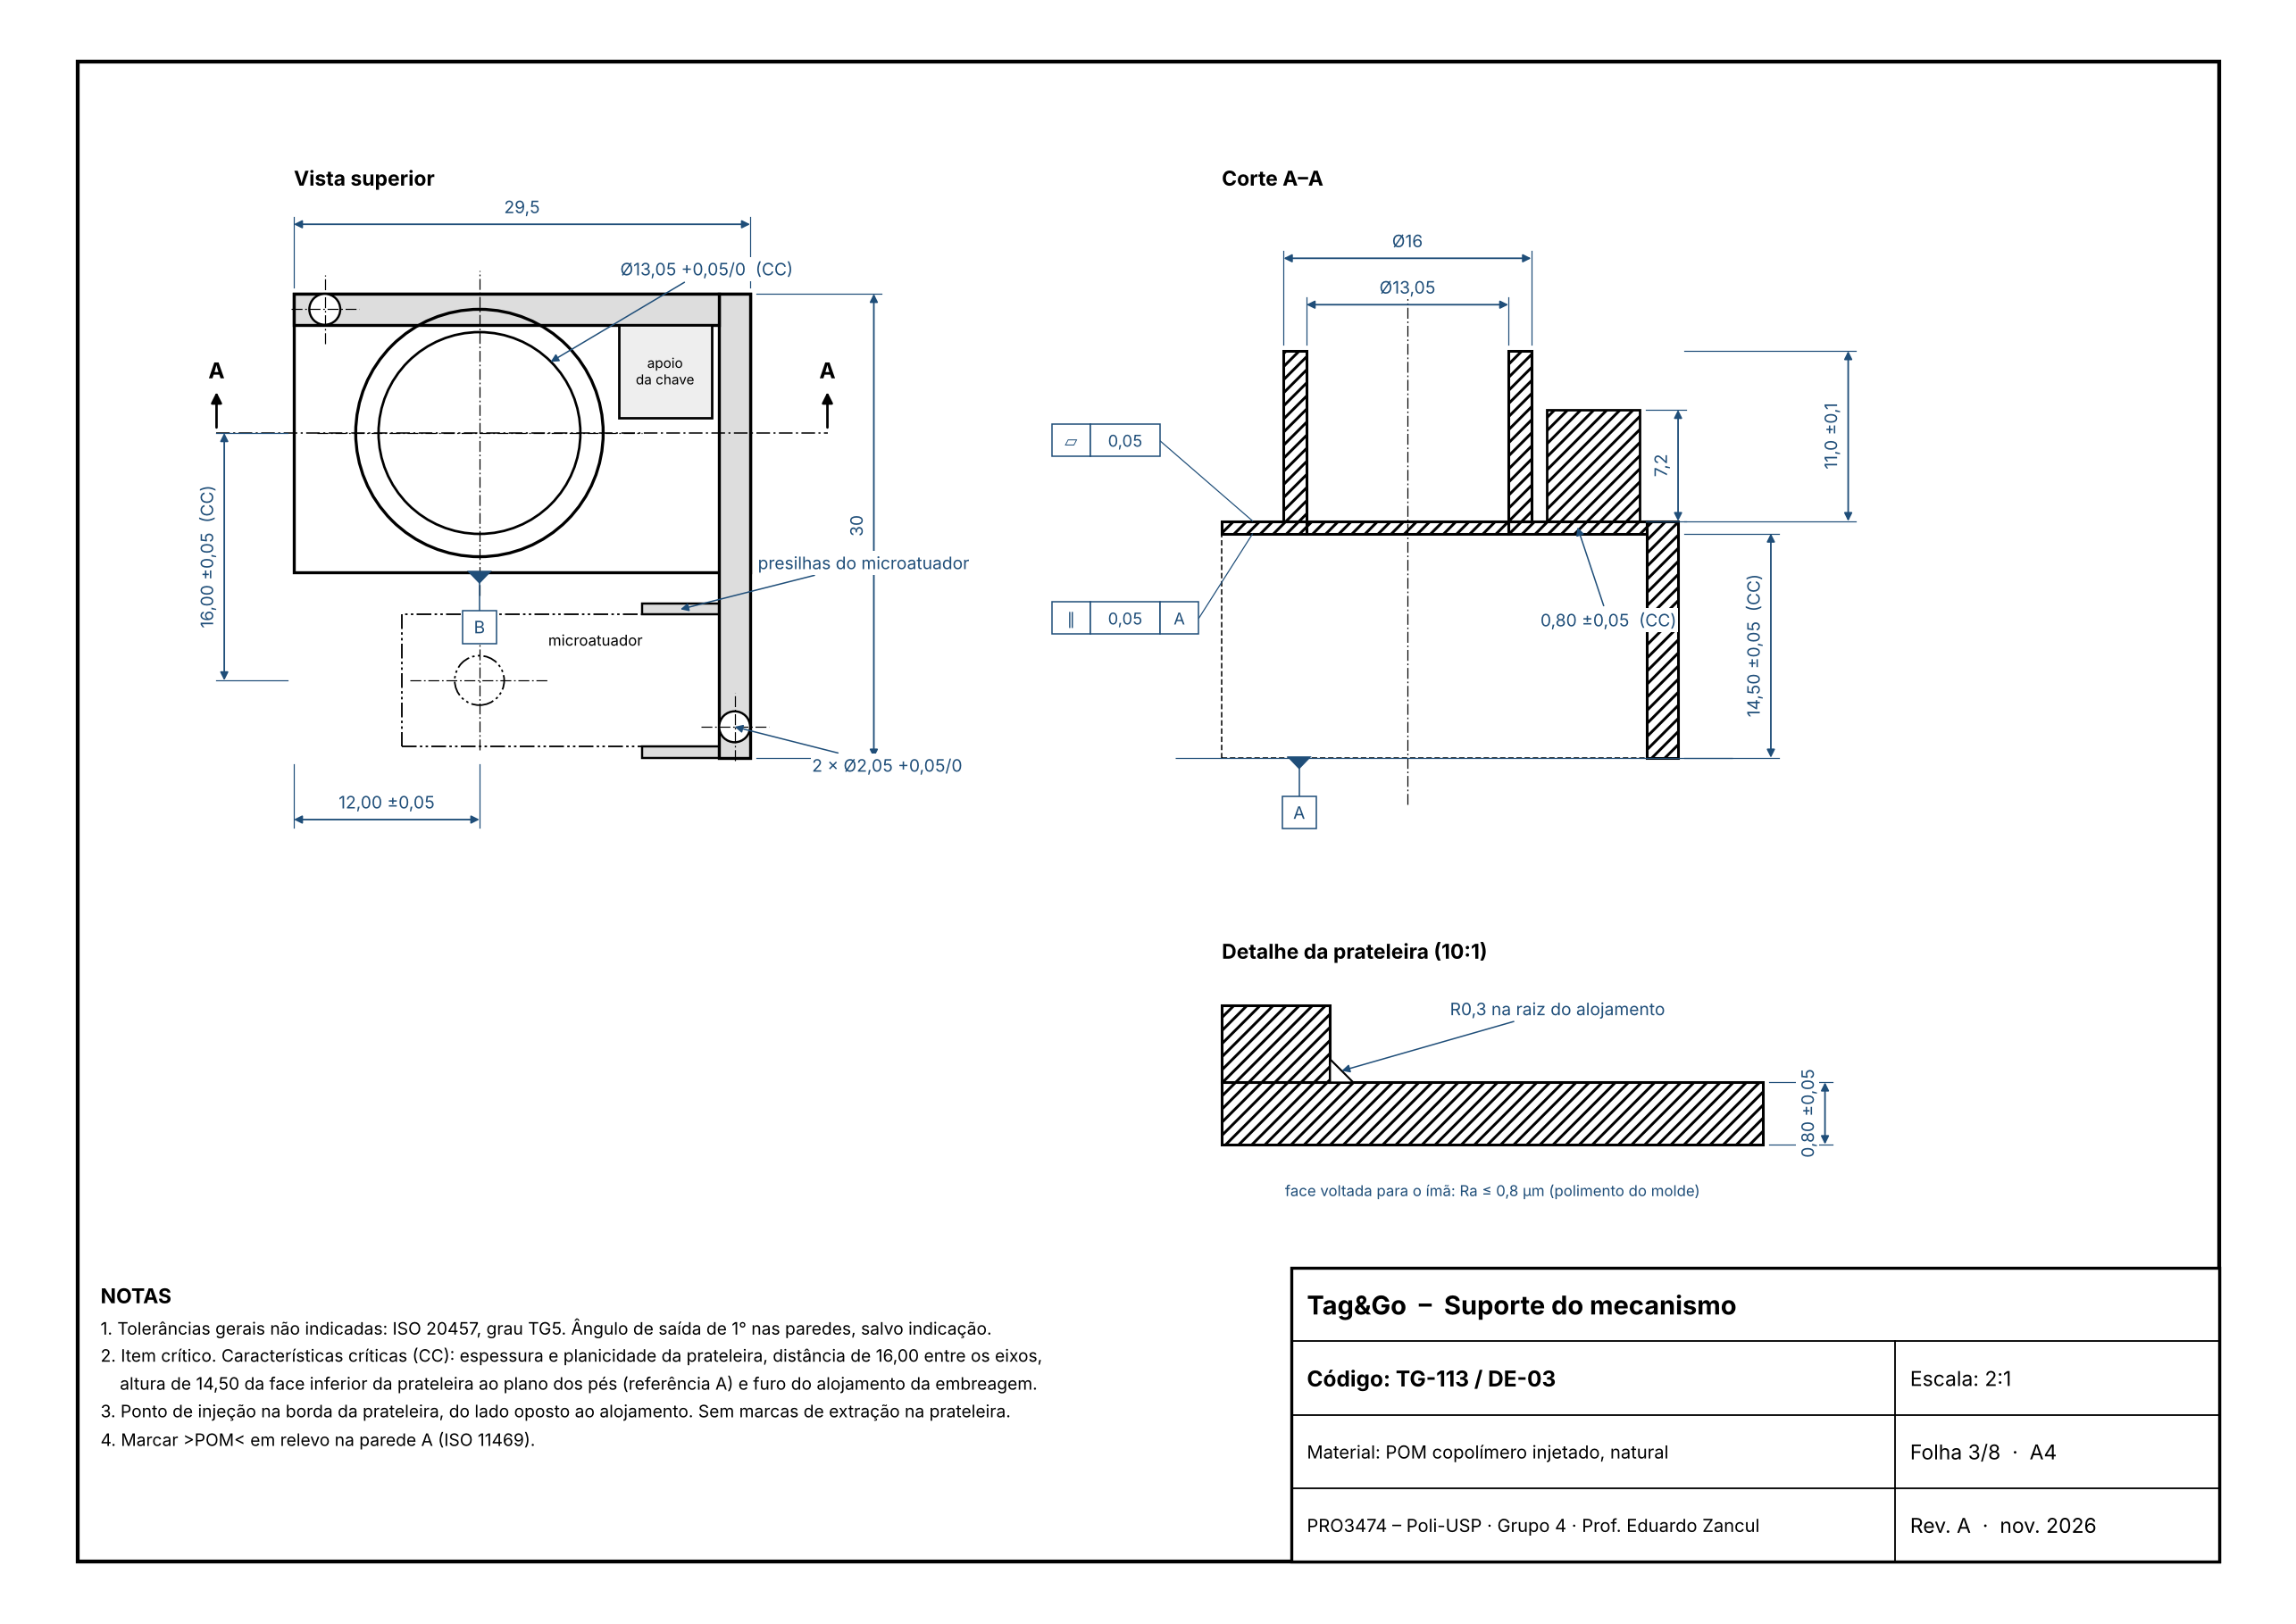
\includegraphics[height=0.86\textheight]{imagens/desenhos_execucao/de03_suporte.png}
    \source{Elaborado pelos autores (2026). Desenho gerado com apoio de ferramenta de IA.}
\end{figure}
\begin{figure}[p]
    \centering
    \caption{Desenho de execução DE-04: corpo da garra, com o pino e o revestimento (TG-211)}
    \label{fig:de04}
    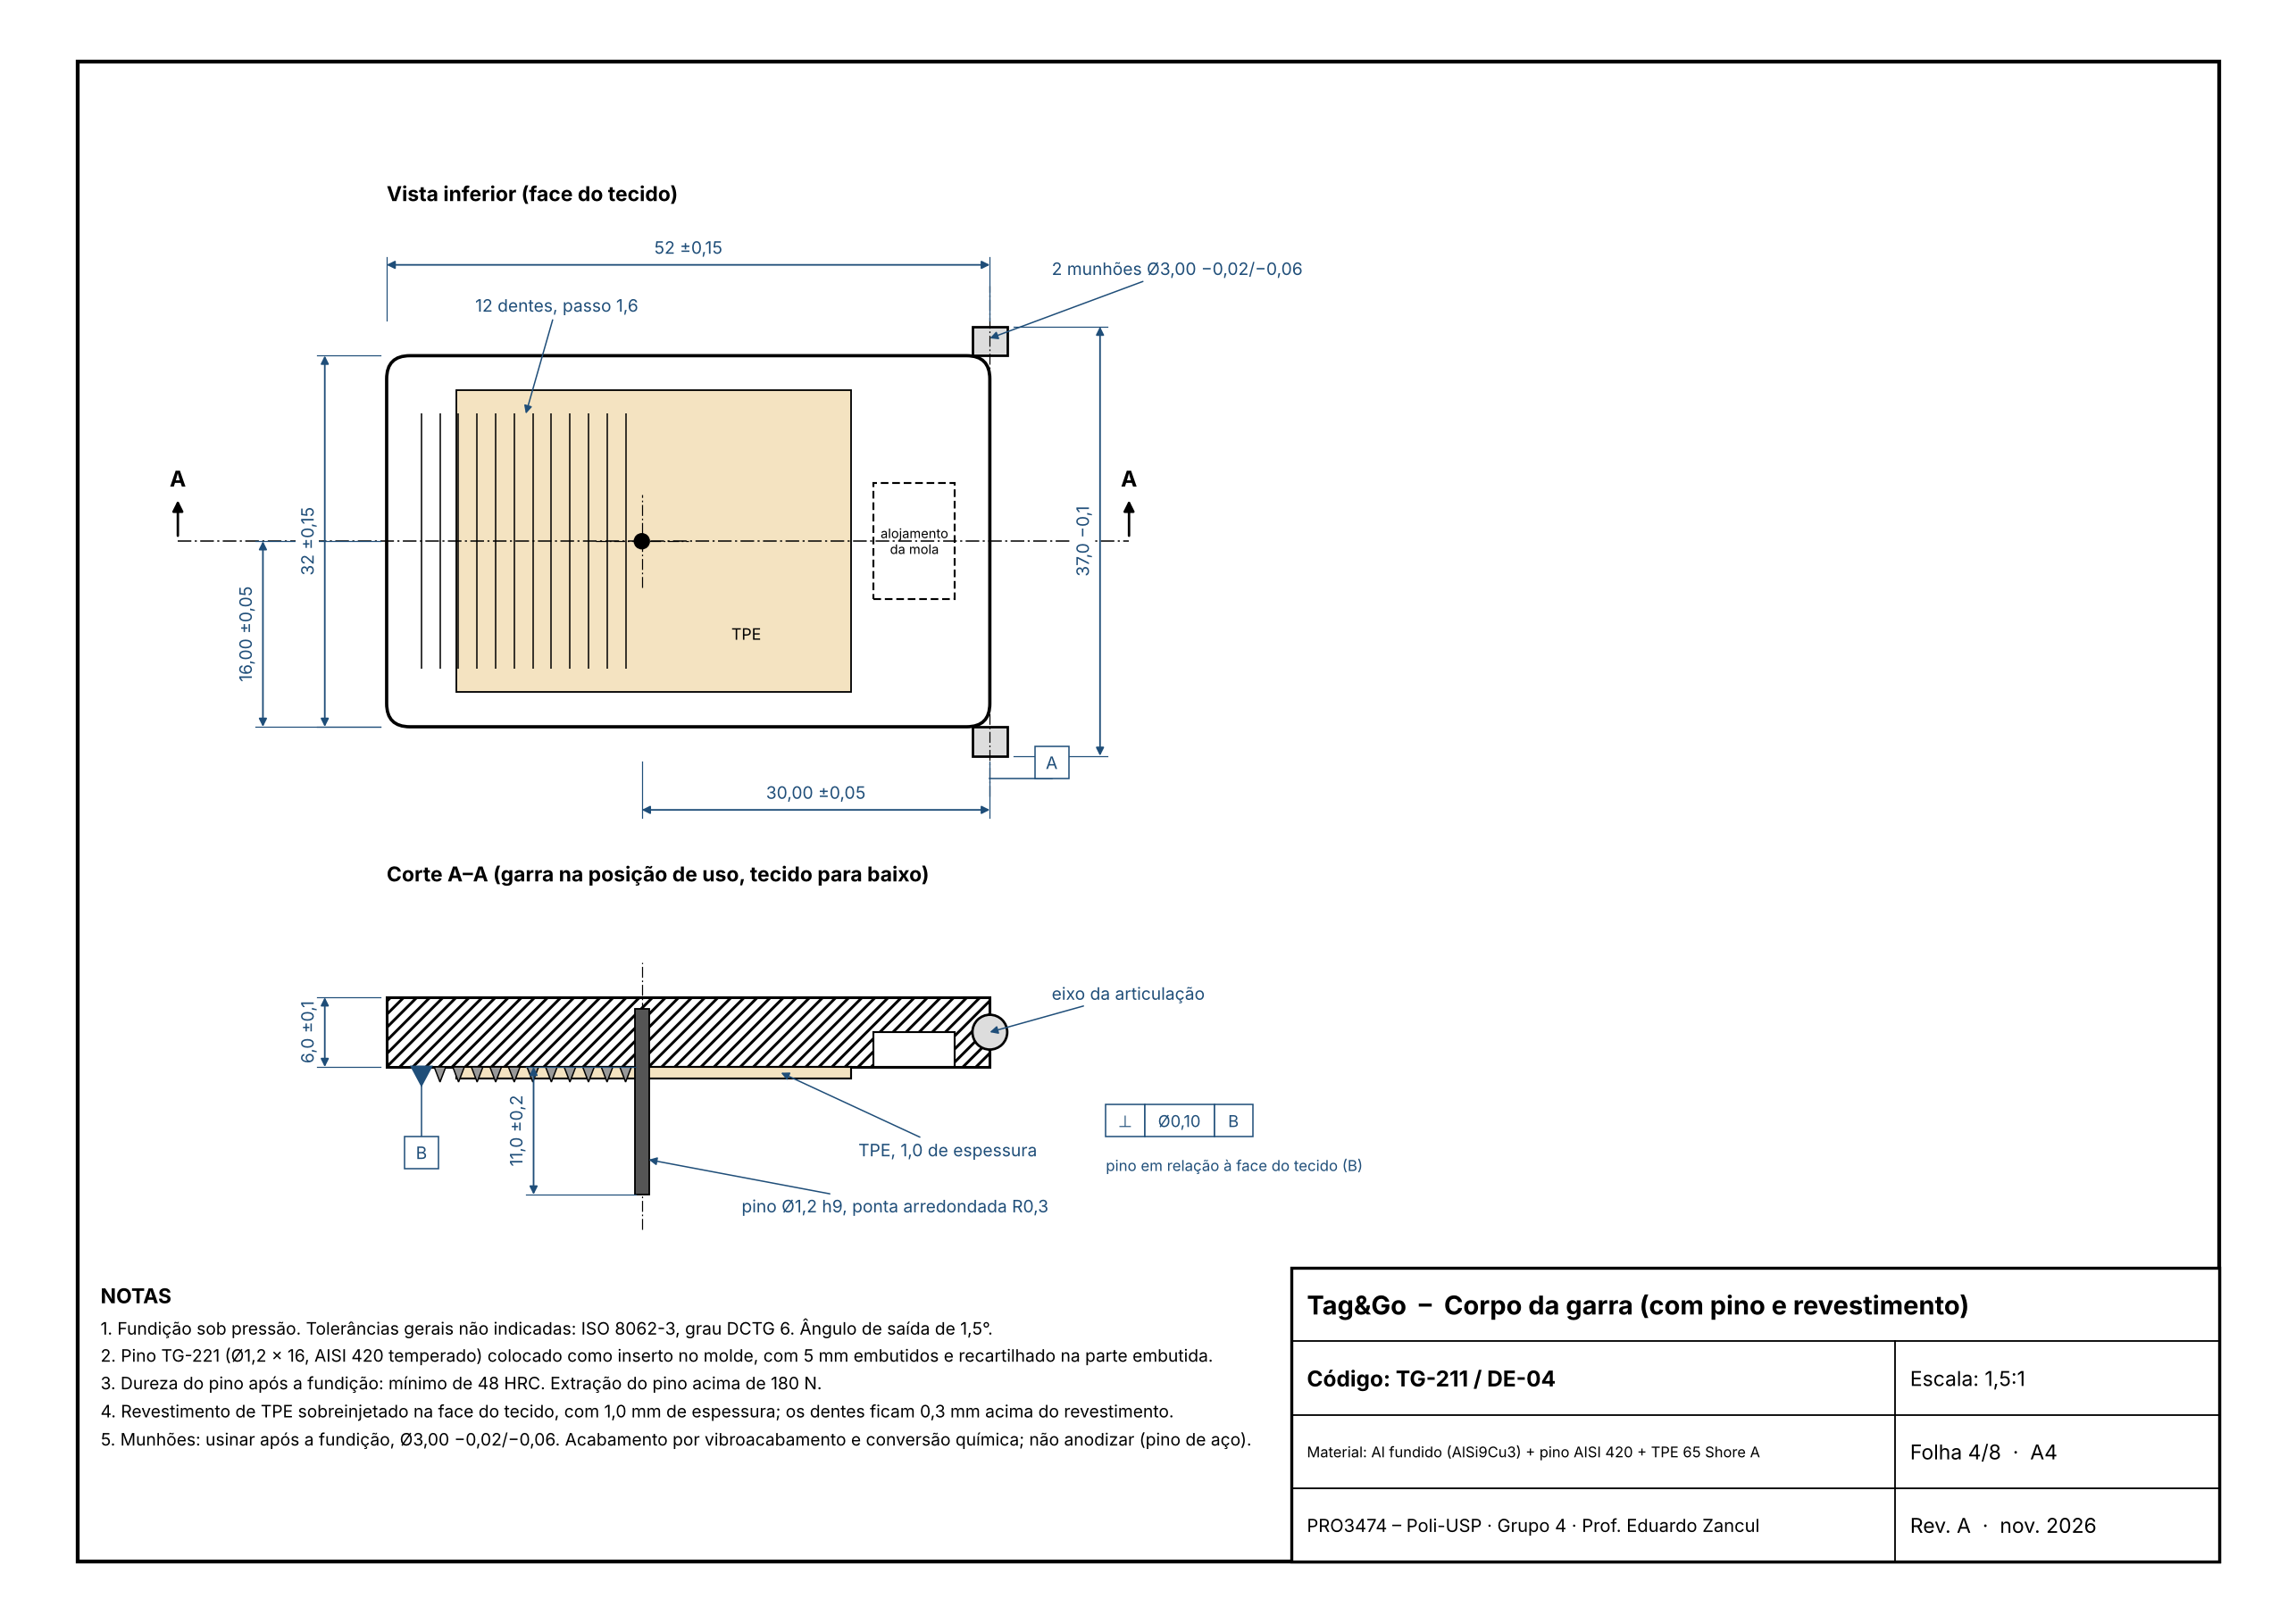
\includegraphics[height=0.86\textheight]{imagens/desenhos_execucao/de04_garra.png}
    \source{Elaborado pelos autores (2026). Desenho gerado com apoio de ferramenta de IA.}
\end{figure}
\begin{figure}[p]
    \centering
    \caption{Desenho de execução DE-05: braço dos ímãs (TG-312)}
    \label{fig:de05}
    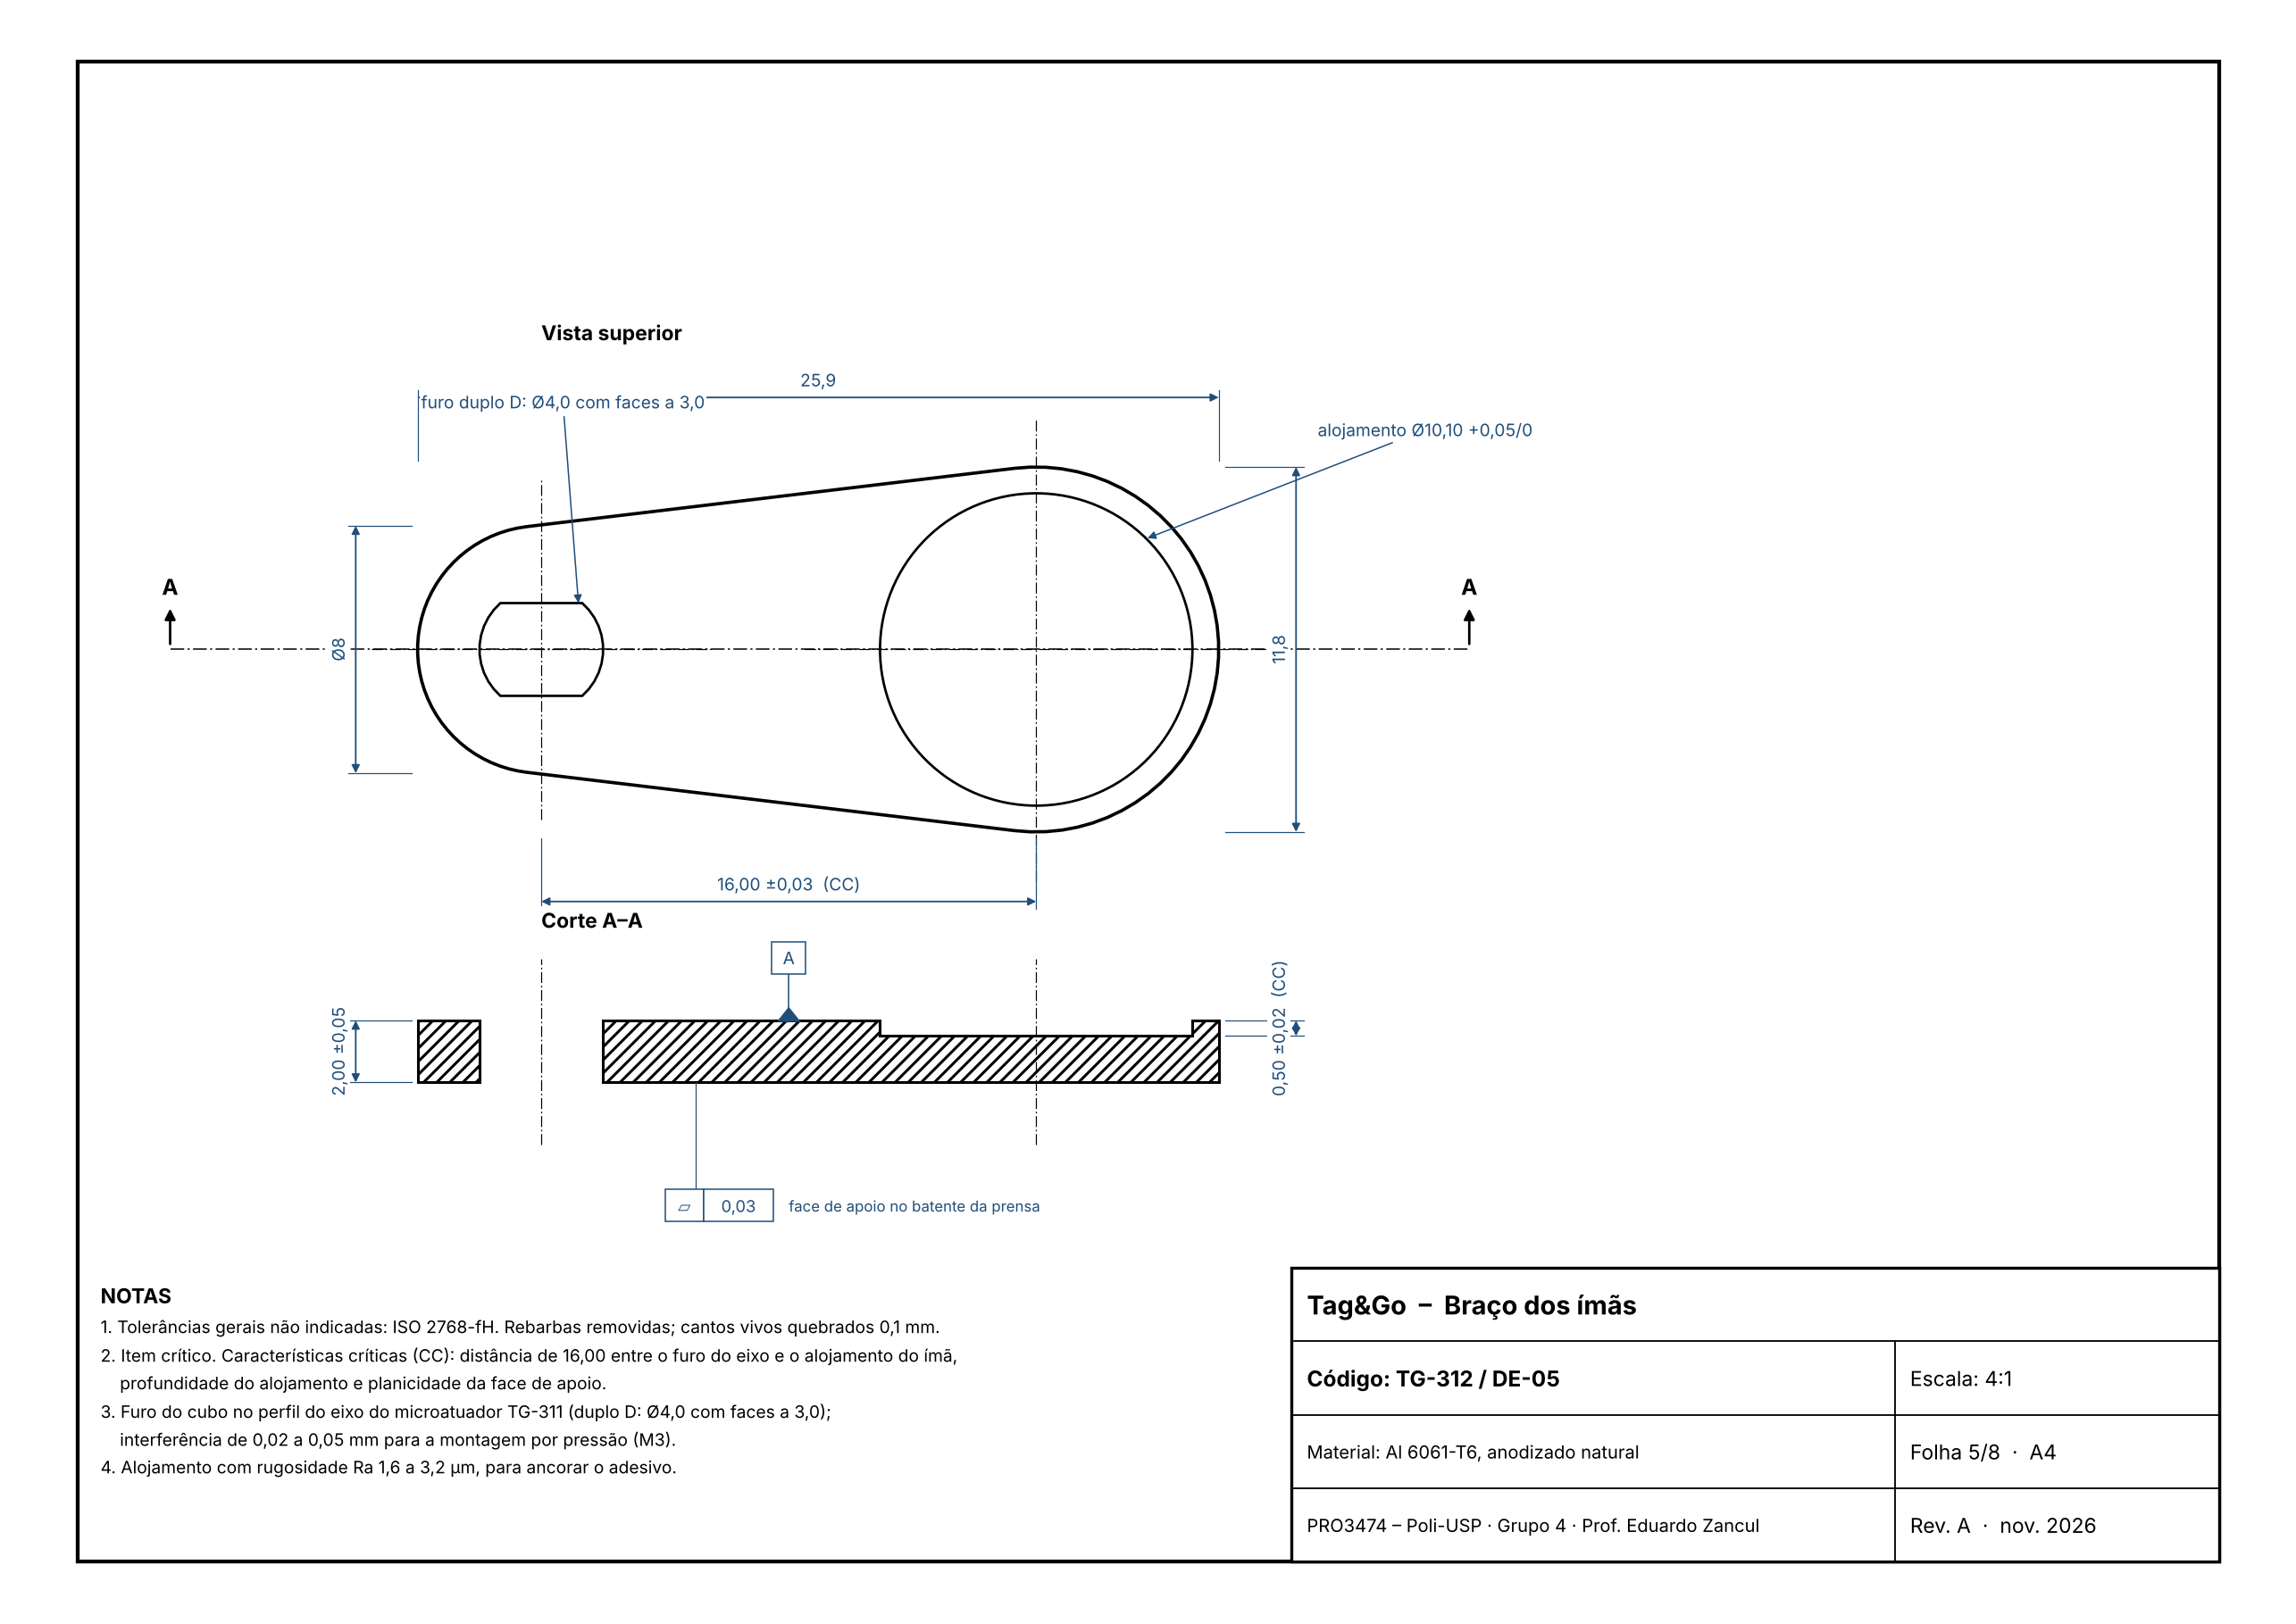
\includegraphics[height=0.86\textheight]{imagens/desenhos_execucao/de05_braco.png}
    \source{Elaborado pelos autores (2026). Desenho gerado com apoio de ferramenta de IA.}
\end{figure}
\begin{figure}[p]
    \centering
    \caption{Desenho de execução DE-06: guia de luz (TG-412) e subconjunto da tampa}
    \label{fig:de06}
    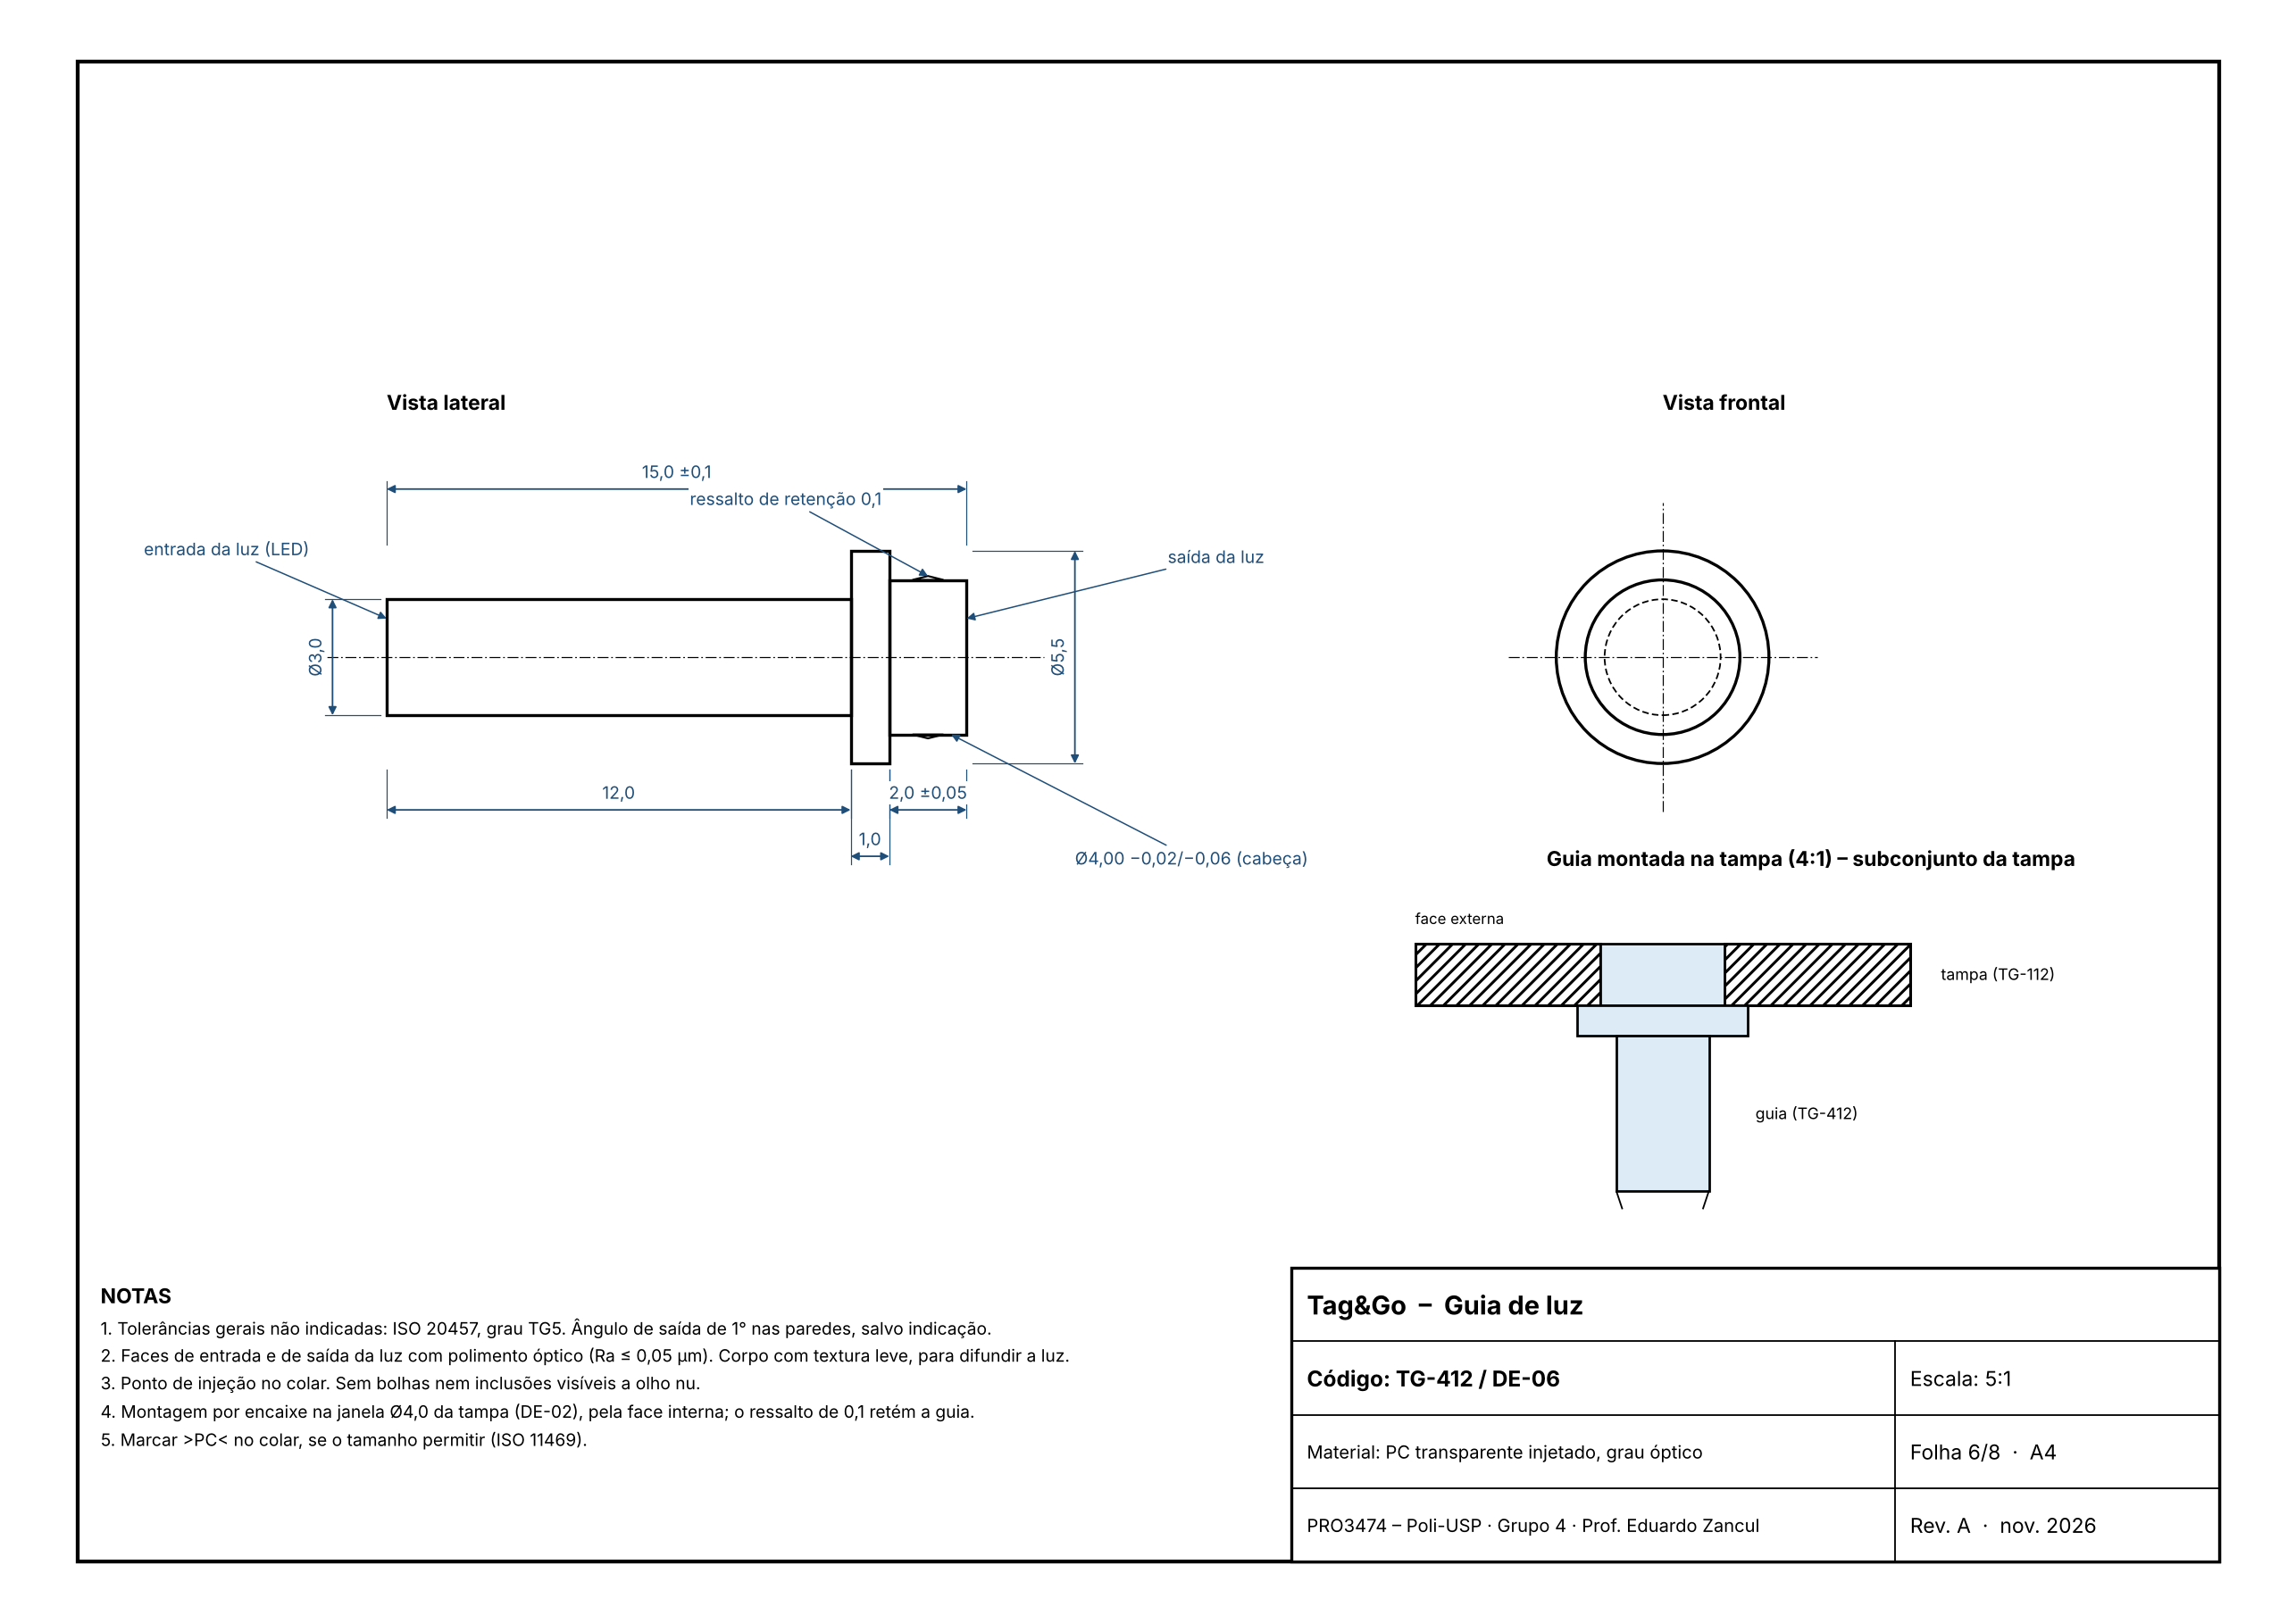
\includegraphics[height=0.86\textheight]{imagens/desenhos_execucao/de06_guia.png}
    \source{Elaborado pelos autores (2026). Desenho gerado com apoio de ferramenta de IA.}
\end{figure}
\begin{figure}[p]
    \centering
    \caption{Desenho de montagem DE-07: subconjunto do mecanismo (SC-01)}
    \label{fig:de07}
    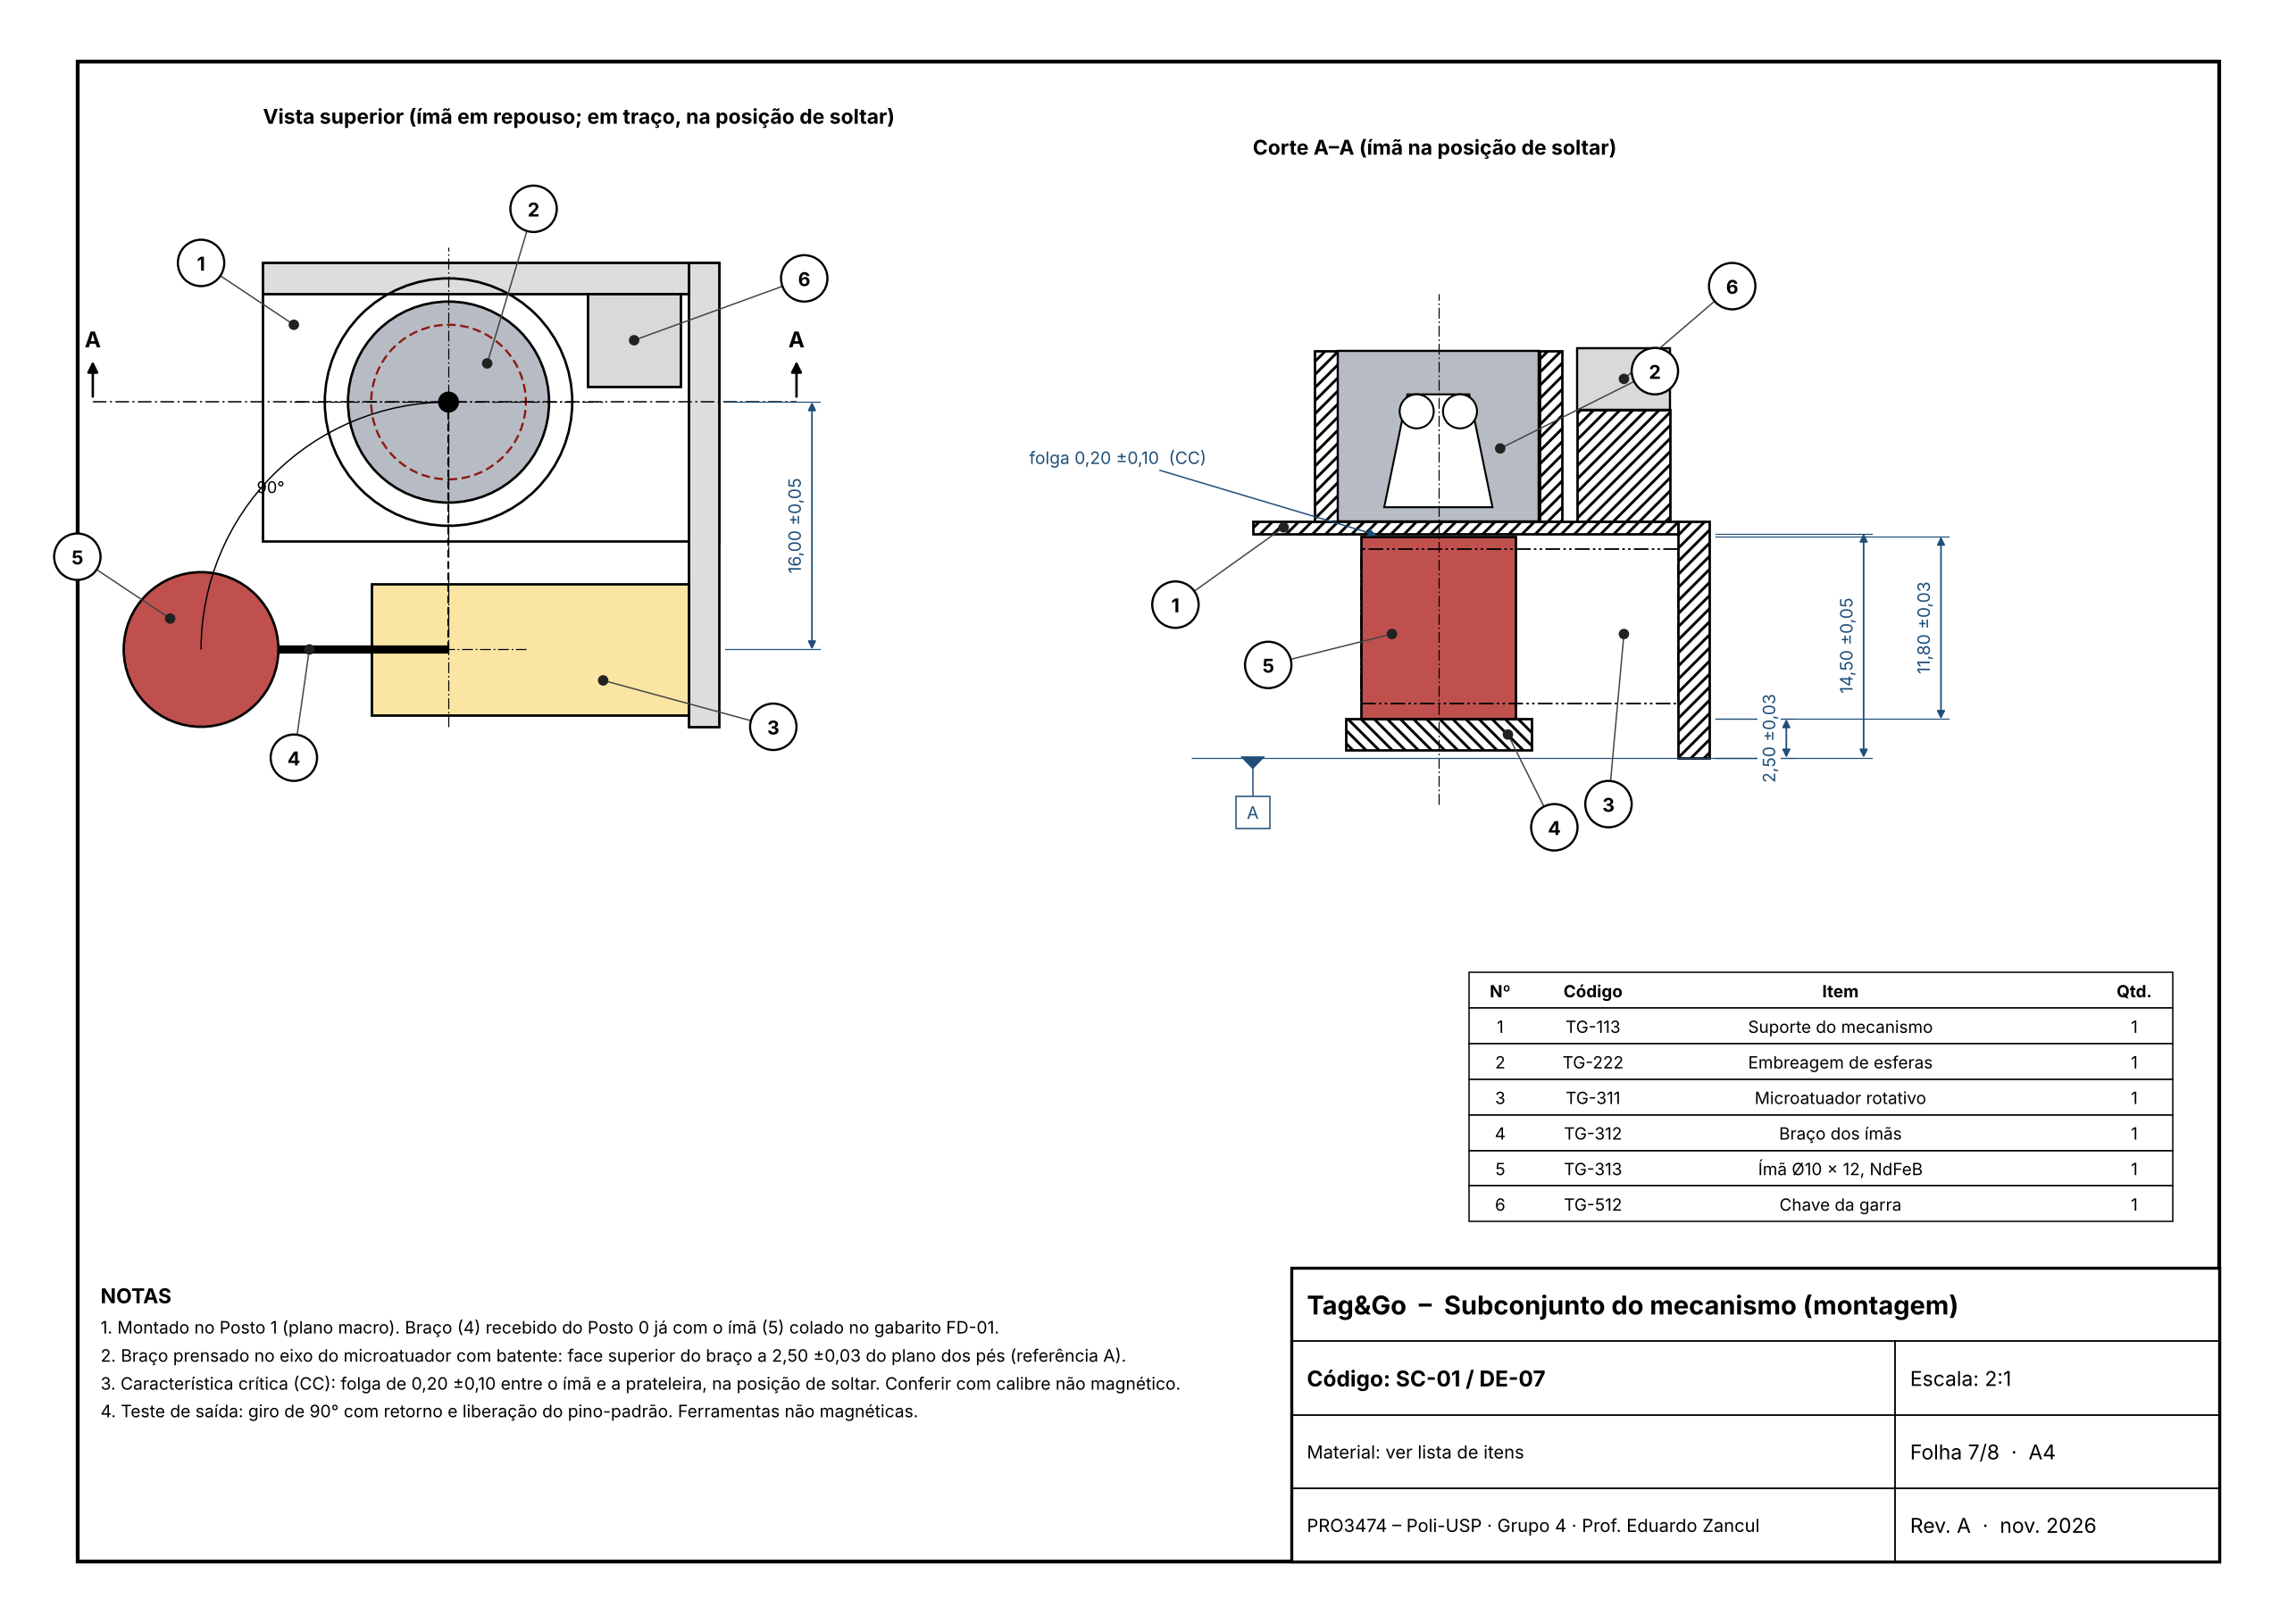
\includegraphics[height=0.86\textheight]{imagens/desenhos_execucao/de07_mecanismo.png}
    \source{Elaborado pelos autores (2026). Desenho gerado com apoio de ferramenta de IA.}
\end{figure}
\end{landscape}
